\section{Structure and thermal protection}
\subsection{Structure}
There are several types of commercial structures. According to the needs of the project, the structure that Astrea is looking for has to be very flexible regarding the placement of the subsystems. It has to adapt to the needs of the project continuously given that the satellite does not have a typical configuration.

A basic schematics can be found in \ref{epsschematics}.

\begin{figure}[H]
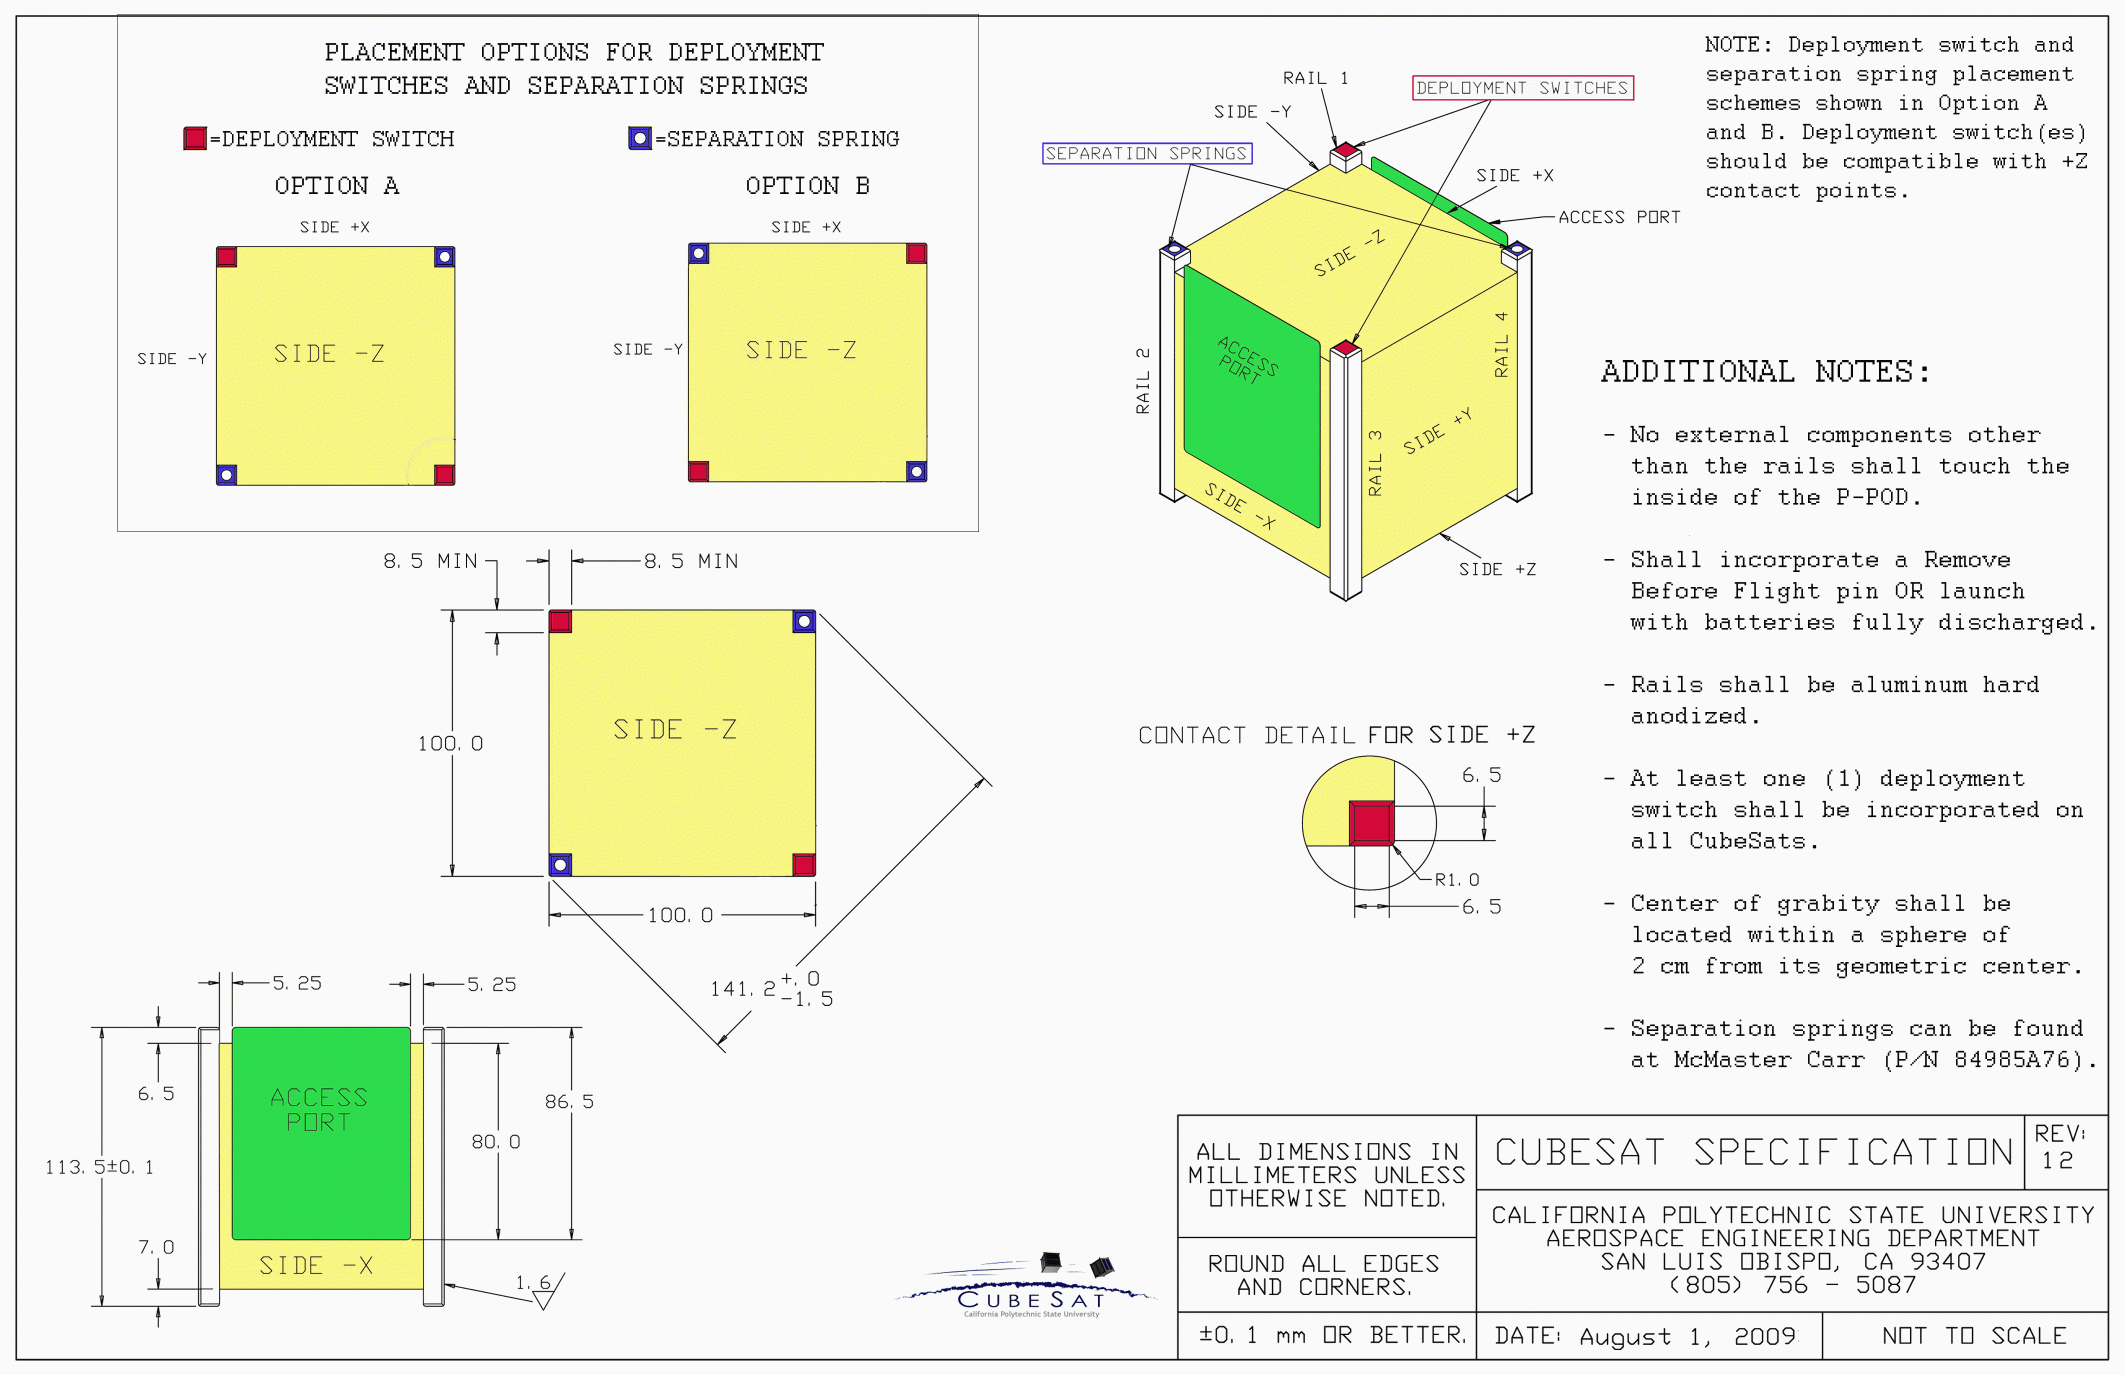
\includegraphics[scale=0.6]{./sections/SatelliteDept/sections/images/CubeSatDesign}
\centering
\caption[Dimensions of a 1U CubeSat]{Dimensions of a 1U CubeSat. Source \cite{CalPoly2014}}
\label{epsschematics}
\end{figure}

Besides this flexibility, several other parameters have to be taken into account. Given that the satellite will work under extreme environmentally conditions, the structure has to withstand space conditions for at least 4 years. Also, the weight should be kept down since there are lots of systems to be placed and the ratio $ mass / satellite $ is limited. Finally, the structure should have a way to place all the subsystems (like holes, \textit{trays}, ...).

The two most interesting options that were considered when the structure had to be chosen are presented in \ref{structureoptions}.

\begin{longtable}{| l | c | c | }
\hline
\rowcolor[gray]{0.80}	\textbf{Brand and model} &  \textbf{Features}     & \textbf{Total price (\euro)}   \\
\hline
\endfirsthead

\rowcolor[gray]{0.85} \textbf{Structure} &  &  \\
	   ~ISIS 3U structure & \makecell{Low mass (304.3g) \\ Highly compatible \\ High temperature range} & 3900 \\
	   \hline
	   ~Gomspace GOMX-Platform & \makecell{High mass (1500g) \\ Comes fully equipped (basic systems) \\ High temperature range} & 11000 \\
	   \hline
\caption{Options studied for the structure}
\label{structureoptions}
\end{longtable}

And the option chosen has been the \textbf{ISIS 3U structure}, as explained in the report.

\subsection{Thermal protection}
The thermal protection system consists of various insulating materials that aim to protect the CubeSat from heat produced by radiation. Currently, the most used element in the aerospace industry is the MultiLayer Insulation (MLI), a set of multiple thin insulation layers. For the satellite, its main objective is to reduce the heat generated by radiation, given that the heat generated by convection or conduction does not have such a high impact on the on-board systems and is also comparatively small with radiation. 

The more layers that the thermal protection has, the more heat is being redressed to the space. An expression for the calculation of the heat flux is presented below:

\begin{equation}
Q=UA\Delta T
\label{eqheatbasic}
\end{equation}

\begin{itemize}
\item $Q$ stands for the radiative heat flow rate between two parallel surfaces
\item $U$ is the global heat transfer coefficient
\item $T$ is the temperature difference between two parallel surfaces
\end{itemize}

The heat transfer coefficient can be derived, theoretically, using the following relation

\begin{equation}
U=4\sigma T^3 \frac{1}{1/\epsilon_{1}+1/ \epsilon_{2}-1}
\label{uderivation}
\end{equation}

If the emissivity is decreased or the number of layers is increased, the heat transfer coefficient is reduced. It means that the system is more insulated, more protected to radiation. Thus, the MLI system is a perfect choice for the satellite: the mass is really low and the insulation obtained is really high (NASA is actually using it for the development of their satellites).Furthermore, this kind of system can also be used as a first protection to dust impacts if the layers are big enough.

Finally, a few options were studied when the thermal protection had to be selected. These options are presented in \ref{thermaloptions}.

\begin{longtable}{| l | c | c | }
\hline
\rowcolor[gray]{0.80}	\textbf{Brand and model} &  \textbf{Features}     & \textbf{Total price (\euro)}   \\
\hline
\endfirsthead
\rowcolor[gray]{0.85} \textbf{Thermal protection} &  &  \\
	   ~Dunmore Aerospace Satkit & \makecell{Lightweight \\ Durability \\ Made for small satellites}& 1000 \\
	   \hline
	   ~Dupont Kapton Aircraft Thermal & \makecell{Lightweight \\ Durability \\ Non-flammable} & 1200 \\
	\hline

\caption{Options studied for the thermal protection}
\label{thermaloptions}
\end{longtable}